% TODO: When to use bullets and when not?

\documentclass{article}

\usepackage{graphicx}
\usepackage{libertine}
\usepackage{libertinust1math}
\usepackage[T1]{fontenc}
%\usepackage{lmodern}
%\usepackage{fontspec}
%\setmainfont{Linux Libertine O}

\usepackage{xcolor}

\definecolor{tempborder}{rgb}{1, 1, 1} % hide temp borders
%\definecolor{tempborder}{rgb}{0.9, 0, 0.9} % show temp borders

\definecolor{strongblue}{rgb}{0.2, 0.3, 0.7} % main theme color

\usepackage{hyperref}
\hypersetup{
    colorlinks=true,
    linkcolor=strongblue,
    filecolor=strongblue,      
    urlcolor=strongblue,
}

\usepackage{pgfpages}
\usepackage{tikz}
\usetikzlibrary{calc}
\usetikzlibrary{matrix}
\usetikzlibrary{positioning}
\usepackage[active,tightpage]{preview}

\pgfdeclarelayer{background}
\pgfsetlayers{background,main}

\begin{document}
\begin{preview}

\def \mywebsite{https://mohnjahoney.github.io}



% Set independent lengths
\newcommand{\sidebarwidth}{6cm} % width of thin sidebar that runs down the side
\newcommand{\headerheight}{4cm} % height of header containing name and contact
\newcommand{\splitradius}{0.5cm} % split circle separates the four quadrants

\newcommand{\sectionpad}{0.35cm} % separation between section header and section and v.v.

\newcommand{\vennrad}{0.5*\headerheight}
\newcommand{\divisionlinewidth}{2pt}
\newcommand{\divisionlinepad}{0.4cm}
\newcommand{\bodytextinnersep}{3pt}

% Compute dependent lengths
% TODO: can I really not do this with \newcommand??
% TODO: need to include line widths?
% TODO: I think inner sep in the text blocks is messing with things.
\pgfmathsetlengthmacro\bodywidth{\pdfpagewidth - \sidebarwidth - \divisionlinewidth}
\pgfmathsetlengthmacro\bodyheight{\pdfpageheight - \headerheight - \divisionlinewidth}
%\pgfmathsetlengthmacro\bodywidth{\pdfpagewidth - \sidebarwidth - 2*\splitradius}
%\pgfmathsetlengthmacro\bodyheight{\pdfpageheight - \headerheight - 2*\splitradius}

%%% TIKZPICTURE
\begin{tikzpicture} [
% Layout stuff
mat/.style={draw=tempborder, rectangle, matrix of nodes, rounded corners, line width=0pt, inner sep=0pt, outer sep=0pt},
sec_title_mat/.style={mat, draw=none, fill=white},%, text width=, text depth=}, % use matrix for organizing each section
sec_body_mat/.style={mat, draw=none, fill=white},%, text width=, text depth=}, % use matrix for organizing each section
sidebar_body_mat/.style={mat, draw=none, fill=strongblue!8!white},%, text width=, text depth=}, % use matrix for organizing each section
% Font stuff
sec_title/.style={font=\Large}, % section title
sec_title_circle/.style={draw=white, circle, line width=2pt, minimum width=0.4cm, anchor=center}, % circles used to demarkate section titles
sec_bold/.style={font=\bfseries\sffamily\normalsize, inner sep=\bodytextinnersep}, % bold "bullets" within each section
sec_text/.style={font=\sffamily\normalsize, inner sep=\bodytextinnersep}, % main text in each section
sidebar_text/.style={font=\sffamily\large, inner sep=\bodytextinnersep}, % main text in each section
%venn/.style={circle, draw=black!60, semithick, minimum size=5cm},
remember picture]

%% draw image
%\node[inner sep=0, opacity=0.3] at (current page)
%%{\includegraphics[width=\paperwidth,height=\paperheight]{poincare_mosaic.pdf}};
%{\includegraphics[width=\paperwidth,height=\paperheight]{me.png}};

%%% Split point - this is the main organizational coordinate
\node[draw=strongblue, circle, line width=2pt, minimum width=2*\splitradius, inner sep=0] (split) at (\sidebarwidth, \pdfpageheight - \headerheight) {};
%\coordinate(split) at (\sidebarwidth, \pdfpageheight - \headerheight);

\draw[strongblue, line width=\divisionlinewidth] (split.center) -- ++(\bodywidth, 0);
\draw[strongblue, line width=2pt] (split.center) -- ++(-\sidebarwidth, 0);
\draw[strongblue, line width=2pt] (split.center) -- ++(0, -\bodyheight);
\draw[strongblue, line width=2pt] (split.center) -- ++(0, \headerheight);

%%% Corner Icon
\begin{scope}
\clip ($(split.center) + (-\vennrad - \divisionlinewidth, \vennrad + \divisionlinewidth)$) circle (\vennrad);
\draw[draw=none, fill=yellow, opacity=1.0] (split.center) circle (1.0*\vennrad);
\end{scope}

%\draw[draw=black!20, line width=2pt] ($(split.center) + (-\vennrad - \divisionlinewidth, \vennrad + \divisionlinewidth)$) circle (\vennrad);
%\draw[draw=black!20, line width=2pt] ($(split.center) + (0, 0)$) +(45:\vennrad) arc (45:225:\vennrad);

% foliation
\begin{scope}
\clip ($(split.center) + (-\vennrad - \divisionlinewidth, \vennrad + \divisionlinewidth)$) circle (\vennrad);

% "normal" foliation
%\foreach \up in {3.1cm, 2.1cm, 1.2cm, 0.5cm, 0cm}{
%\filldraw[draw=black!50, semithick, fill=green, fill opacity=0.1] ($(split.center) + (-3*\vennrad, \up)$) -- ++(1.666*\vennrad + \up, 0cm) -- ++(\vennrad,-\vennrad) -- ++(0cm, -\vennrad) -- ++(-3*\vennrad, 0cm) -- cycle;

% fancy foliation
% start at center, move radially to edge, back up diagonally, then draw
%\foreach \up in {2.0cm, 1.6cm, 1.2cm, 0.8cm, 0.4cm, 0cm}{
%\foreach \up in {5, 4, 3, 2, 1, 0}{
%\filldraw[draw=black!50, line width=0.02*\up*1cm, fill=green, fill opacity=0.06] ($(split.center) + (-3*\vennrad, \up * 0.1cm)$) -- ++(1.666*\vennrad + 0.1*\up * 1cm, 0cm) -- ++(\vennrad,-\vennrad) -- ++(0cm, -\vennrad) -- ++(-3*\vennrad, 0cm) -- cycle;
\foreach \up in {7, 6, 5, 4, 3, 2, 1}{
\filldraw[draw=black!50, line width=0.02cm, fill=green, fill opacity=0.1] ($(split.center) + (-\vennrad, 0)$) -- (split.center) -- ++(\up*12+90:\vennrad) -- ++(-2*\vennrad, 0) -- ++(0, -2*\vennrad) -- cycle;
\draw[draw=black!20, line width=4pt] ($(split.center) + (-2*\vennrad, \vennrad)$) arc (180:0:\vennrad);
%\draw[] ($(split.center) + (-\vennrad, 0)$) arc 

% TODO: could use the control points to make foliation curved
%\filldraw[draw=black!60, semithick, fill=blue, fill opacity=0.1] ($(split.center) + (-\vennrad, \up)$) .. controls ++(-2,-2+\up) and (-1,0+\up) ..  (2,-1+\up) -- (3,0) -- (3,-5) -- (-3,-5) --   cycle;
}
\end{scope}

%%% Profile
\matrix[sec_body_mat, anchor=south west, line width=2pt, draw=none,
column 1/.style={sec_text, font=\Large, text width=0.9*\bodywidth}] (profile) at ($(split.center) + (\divisionlinepad, 2*\sectionpad)$){
\emph{
%I am a lifelong learner who cares deeply about our world and the beings in it.
I love to create, combine, and recontextualize.
%I am a vigorous skeptic, but I'm always on your side.
}\\
%\emph{
%I'm a rad dad who endeavors to make the world a fizzier place. 
%A physicist by training and jazz saxophonist by night, I approach the world with both an analytic mind and a the desire for a deep pocket.
%}\\
};

%\matrix[sec_title_mat, anchor=south west,
%row 1/.style={sec_title, anchor=center}] (profile_title) at ($(profile.north west) + (0.0cm, +\sectionpad)$) {
%\node[sec_title_circle, draw=black!20, fill=green, fill opacity=0.3 ] {};&
%~~PROFILE~~&
%\node[sec_title_circle] {};\\
%};

%%% NAME other design
\node[color=white, fill=strongblue, draw=none, line width=2pt, font=\huge, scale=1.8, rounded corners, anchor=south west] (name) at ($(profile.north west) + (0, 2*\sectionpad)$) {\textcolor{white}{~~~~John R. Mahoney~~~~}};
%\node[color=white, fill=strongblue, font=\huge, scale=2.0, anchor=south west] (name) at ($(profile_title.north west) + (0, +\sectionpad)$) {\textcolor{white}{John R. Mahoney}};

%%% Communication Skills
\matrix[sec_title_mat, anchor=north west,
row 1/.style={sec_title, anchor=center}] (communication_skills_title) at ($(split.center) + (\divisionlinepad, -2*\sectionpad)$) {
\node[sec_title_circle, draw=black!20, fill=green, fill opacity=0.3] {};&
~~COMMUNICATION SKILLS~~&
\node[sec_title_circle] {};\\
};

\matrix[sec_body_mat, anchor=north west, 
column 1/.style={sec_bold, text width=0.2*\bodywidth},
column 2/.style={sec_text, text width=0.8*\bodywidth - \divisionlinepad - 4*\bodytextinnersep}] (communication_skills) at ($(communication_skills_title.south west) + (0.0, -\sectionpad)$){
Written: &  Wrote and co-authored over 25 papers published in high quality journals (PRL, PRX, PRA, PRE, CHAOS, J. Stat Phys.). Edited multiple articles for colleagues.
%Refereed for several journals.
Read about:
\href{https://mohnjahoney.github.io/pdfs/Times_Barbed_Arrow.pdf}{prediction}, 
\href{https://mohnjahoney.github.io/pdfs/A_Turnstile_Mechanism_For_Fronts_Propagating_In_Fluid_Flows.pdf}{reacting fluids}, 
\href{https://mohnjahoney.github.io/pdfs/Occams_Quantum_Strop.pdf}{quantum information}.\\
Verbal: & Designed and delivered over 35 talks and posters including:
Quantum Info Workshop at Nanyang Technical University, Singapore;
Conference on Complex Systems, Amsterdam;
CHAOS15 at Henri Poincar\'e Institute, Paris;
Oberwolfach, Germany (awarded \href{https://mohnjahoney.github.io/pdfs/posters/Oberwolfach2014.pdf}{``best poster''});
%International Conference on Flow Dynamics, Sendai, Japan
%International Conference on Nonlinear Science and Complexity, Budapest, Hungary
% TODO: add "Listen to: link to a talk I've given."
\\
Visual: & Value aesthetic communication. Created scientifically advanced visual representation of reacting flow topology. Promoted and taught use of Venn diagrams for information theory. Often discover and appreciate connection between art and science.
Look at:
\href{https://mohnjahoney.github.io/images/burning_front_topology.png}{topology of reacting flows}, 
\href{https://mohnjahoney.github.io/images/FoliationCryptic.pdf}{info diagram}, 
%\href{https://mohnjahoney.github.io/images/quantum_strop_nemo.png}{quantum compression},
\href{https://mohnjahoney.github.io/images/poincare_mosaic.pdf}{Poincar\'e art}.\\
% TODO: add a video - maybe a BIM animation
%\phantom{blank} & Examples: \href{https://mohnjahoney.github.io/images/burning_front_topology.png}{A}, \href{https://mohnjahoney.github.io/images/quantum_strop_nemo.png}{B}, \href{https://mohnjahoney.github.io/images/poincare_mosaic.pdf}{C}\\
%\phantom{blank} & \node[draw=none] () {
%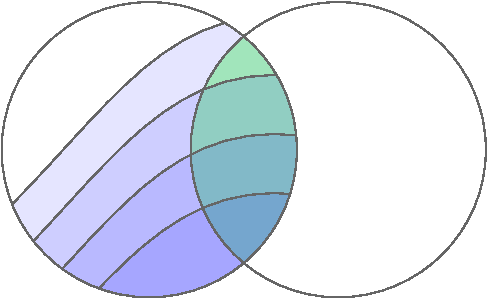
\includegraphics[width=2cm]{FoliationMarkov.pdf}
%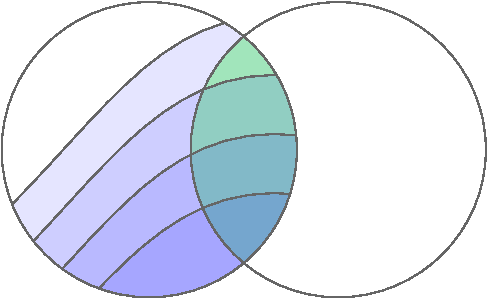
\includegraphics[width=2cm]{FoliationMarkov.pdf}};\\
};

%%% Analytic Skills
\matrix[sec_title_mat, anchor=north west,
row 1/.style={sec_title, anchor=center}] (analytic_skills_title) at ($(communication_skills.south west) + (0.0cm, -2*\sectionpad)$) {
\node[sec_title_circle, draw=black!20, fill=green, fill opacity=0.3] {};&
~~ANALYTIC SKILLS~~&
\node[sec_title_circle] {};\\
};

\matrix[sec_body_mat, anchor=north west, 
column 1/.style={sec_bold, text width=0.2*\bodywidth},
column 2/.style={sec_text, text width=0.8*\bodywidth - \divisionlinepad - 4*\bodytextinnersep}] (analytic_skills) at ($(analytic_skills_title.south west) + (0.0cm, -\sectionpad)$) {
Research: & Connected my work on reacting fluids to existing fields: invariant manifolds, FT Lyapunov exponents, ARD equation, catastrophe theory, vehicle path planning, differential geometry.\\
Critical Thinking: & Reframed an assumption in the literature to build a fruitful research avenue - \textit{crypticity and cryptic order}. \\
Data: & Created Python pipeline for data on diabetes patients: clean, process, analyze (multiple pair lagged regression), visualize. \\
};


%%% Work Experience
\matrix[sec_title_mat, anchor=north west,
row 1/.style={sec_title, anchor=center}] (work_experience_title) at ($(analytic_skills.south west) + (0.0cm, -2*\sectionpad)$) {
\node[sec_title_circle, draw=black!20, fill=green, fill opacity=0.3] {};&
~~WORK EXPERIENCE~~&
\node[sec_title_circle] {};\\
};

\matrix[sec_body_mat, anchor=north west, 
column 1/.style={sec_bold, text width=0.2*\bodywidth},
column 2/.style={sec_text, text width=0.8*\bodywidth - \divisionlinepad - 4*\bodytextinnersep}
] (work_experience) at ($(work_experience_title.south west) + (0.0cm, -\sectionpad)$) {
Fall 2020&Math Specialist: UC Davis\\
Summer 2020&Course Designer and Instructor: UC Davis\\
Oct 2019&Math Lecturer: Napa Valley College\\
Spring 2019&Physics Lecturer: UC Davis\\
Fall 2018&Math Lecturer: CSU Maritime\\
2017-2018&Consultant: Dept. Biomedical Informatics, Columbia University\\
Fall 2017&Spring 2018, Math Lecturer: UC Davis\\
2015-2017&Project Scientist: UC Davis\\
2010-2015&Postdoctoral Scholar: UC Merced\\
};


%%% Education
\matrix[sec_title_mat, anchor=north west,
row 1/.style={sec_title, anchor=center}] (education_title) at ($(work_experience.south west) + (0.0cm, -2*\sectionpad)$) {
\node[sec_title_circle, draw=black!20, fill=green, fill opacity=0.3] {};&
~~EDUCATION~~&
\node[sec_title_circle] {};\\
};

\matrix[sec_body_mat, anchor=north west,
column 1/.style={sec_text, anchor=west}, text width=1.0*\bodywidth - \divisionlinepad - 2*\bodytextinnersep] (education) at ($(education_title.south west) + (0.0cm, -\sectionpad)$) {
Ph.D. in Physics, UC Davis, advisor: James P. Crutchfield\\
%�Extensions of the Theory of Computational Mechanics�
B.S. in Physics and Mathematics, CSU Chico\\
attended Williams College for Physics, Mathematics and Music\\
};


%%%%%%%%%%%
% Sidebar
%%%%%%%%%%%

%%% Programming Skills
\matrix[sec_title_mat, anchor=north east,
row 1/.style={sec_title, anchor=center}] (programming_skills_title) at ($(split.center) + (-\divisionlinepad, -2*\sectionpad)$) {
\node[sec_title_circle] {};&
~~PROGRAMMING~~&
\node[sec_title_circle] {};\\
};

%column 1/.style={font=\bfseries\Large, text width=0.2*\bodywidth},
%column 2/.style={text width=0.7*\bodywidth}
\matrix[sidebar_body_mat, anchor=north east, text width=1.0*\sidebarwidth - \divisionlinepad - 2*\bodytextinnersep, align=right, 
column 1/.style={sidebar_text, anchor=west}] (programming_skills) at ($(programming_skills_title.south east) + (0.0cm, -\sectionpad)$) {
Python: np, sp, mpl, pd\\
GUI / interactive\\
git, \LaTeX, beamer, tikz\\
ipython, Jupyter, VS Code\\
MATLAB\\
Mac OS, UNIX\\
};

%%% Interpersonal Skills
\matrix[sec_title_mat, anchor=north east,
row 1/.style={sec_title, anchor=center}] (interpersonal_skills_title) at ($(programming_skills.south east) + (0.0cm, -2*\sectionpad)$) {
\node[sec_title_circle] {};&
~~INTERPERSONAL~~&
\node[sec_title_circle] {};\\
};

\matrix[sidebar_body_mat, anchor=north east, text width=1.0*\sidebarwidth  - \divisionlinepad - 2*\bodytextinnersep, align=right,
column 1/.style={sidebar_text}] (interpersonal_skills) at ($(interpersonal_skills_title.south east) + (0.0cm, -\sectionpad)$) {
Excellent listener\\
Flexible and creative\\
Work well in close-knit teams\\
Independent worker\\
Thoughtful mentor\\%: (3 PhD, 7 undergrads)\\
};


%%% Projects
\matrix[sec_title_mat, anchor=north east,
row 1/.style={sec_title, anchor=center}] (projects_title) at ($(interpersonal_skills.south east) + (0.0cm, -2*\sectionpad)$) {
\node[sec_title_circle] {};&
~~PROJECTS~~&
\node[sec_title_circle] {};\\
};

\matrix[sidebar_body_mat, anchor=north east, text width=1.0*\sidebarwidth - \divisionlinepad - 2*\bodytextinnersep, align=right,
column 1/.style={sidebar_text}] (projects) at ($(projects_title.south east) + (0.0cm, -\sectionpad)$) {
\href{https://github.com/mohnjahoney/magnacules}{Python \& Physics course}\\
\href{link}{Burning Invariant Manifolds}\\
\href{link}{CMPy} contributor\\
\href{https://github.com/mohnjahoney/simpsons_paradox}{Simpson's Paradox}\\
\href{link}{timesquare}\\
\href{https://github.com/mohnjahoney/resume}{resum\`e template}\\
};


%%% INTERESTS
\matrix[sec_title_mat, anchor=north east,
row 1/.style={sec_title, anchor=center}] (interests_title) at ($(projects.south east) + (0.0cm, -2*\sectionpad)$) {
\node[sec_title_circle] {};&
~~INTERESTS~~&
\node[sec_title_circle] {};\\
};

\matrix[sidebar_body_mat, anchor=north east, text width=1.0*\sidebarwidth - \divisionlinepad - 2*\bodytextinnersep, align=right,
column 1/.style={sidebar_text}] (interests) at ($(interests_title.south east) + (0.0cm, -\sectionpad)$) {
jazz saxophone and piano\\
soccer, tennis, and hiking\\
cooking delicious food!\\
};


\matrix[mat, anchor=north east, sidebar_text,
inner sep=\bodytextinnersep, draw=none, line width=2pt, fill=white, fill opacity=0.5, draw opacity=1.0, text opacity=1.0] (contact) at ($(interests.south east) + (0.0cm, -2*\sectionpad)$) {
mohnjahoney@gmail.com\\
(530) 601-0524\\
\href{\mywebsite}{mohnjahoney.github.io}\\
\node[draw=none, line width=3pt, rectangle] (gh) {
\href{https://github.com/mohnjahoney}{
\includegraphics[width=0.8cm]{github.pdf}}
\quad
\href{https://www.linkedin.com/in/johnmahoney3}{
\includegraphics[width=0.8cm]{LI-In-Bug.png}}
};\\
};


\end{tikzpicture}
\end{preview}
\end{document}
